\chapter{Generative Diffeomorphic Deformation Models}
Generative models have been successfully applied in a wide range of medical image analysis tasks such as TODO list some applications. 

Diffeomorphic deformations of particular interest due to the organic nature and modeling of gradual changes
Contrasts with additive changes in e.g. classic CNN

Diffeomorphic transformations are differentiable and invertible and therefore topology preserving

diffeomorphism important because of understanding/grasp of processes


In this section, we discuss the general architecture of our model. We first examine the brain registration model proposed in \cite{voxelmorph} and then discuss our adaptation for the generative brain aging task.

\section{Diffeomorphic Image Registration}
\label{chap:voxelmorph}
In medical imaging, deformable image registration tackles the problem of warping one image onto another. More formally, given two scans $x$ and $y$, the aim is to find a deformation function $\Phi$ such that $x \circ \Phi$ is similar to $y$.

\subsection{Voxelmorph}
Dalca et al propose a deep learning architecture to learn such a mapping for 3-dimensional MRI brain data. Specifically, given $x$ and $y$ the model generates a stationary velocity field $v$ which defines the deformation ${\Phi : \R^3 \rightarrow \R^3}$ mapping $x$ to $y$ through the ordinary differential equation (ODE)
\begin{equation} \label{eq:voxODE}
	\frac{\partial \Phi^{(t)}}{\partial t} = v(\Phi^{(t)})
\end{equation}

where $\Phi^{(0)} = id$ is the identity transformation and t is time.
The final deformation field $\Phi^{(1)}$ is then obtained by integrating the field $v$ over time $t = [0, 1]$, which is computed numerically using the scaling and squaring method.

In group theory, $v$ is a member of the Lie algebra and is exponentiated to produce $\Phi^{(1)} = \exp(v)$.
The collection $\{\Phi^{(t)}\}_{t \; \in \; [0,1]}$ forms a one-parameter subgroup of diffeomorphisms and therefore for any scalars $t$ and $t'$ we have 
\begin{equation} \label{eq:voxoneparamsubgroup}
	\exp((t + t')v) = \exp(tv) \circ \exp(t'v)
\end{equation}

where $\circ$ is a composition map associated with the Lie group. Consequently, we can then use the recurrence
\begin{equation} \label{eq:voxrecurrence}
	\Phi^{(1/2^{(t-1)})} = \Phi^{(1/2^{t})} \circ \Phi^{(1/2^{t})}
\end{equation}

starting from $\Phi^{(1/2^T)}$ to obtain $\Phi^{(1)} = \Phi^{(1/2)} \circ \Phi^{(1/2)}$ where $T$ is chosen such that $v \approx 0$.

The model uses a variational inference method to generate a stationary displacement field $z$ which defines the deformation $\Phi_z$ through the ODE (\ref{eq:voxODE}). The prior probabilty of $z$ is modeled as
\begin{equation}
	p(z) = \mathcal{N}(z; 0, \Sigma_z)
\end{equation}

Spatial smoothness of z is is encouraged by letting ${\Sigma_z^{-1} = \Lambda_z = \lambda L}$ where $\Lambda_z$ is a precision matrix, $L$ is the Laplacian of a neighborhood graph defined as $L = D - A$, with graph degree matrix $D$ and voxel adjacency matrix $A$, and $\lambda$ denotes a parameter controlling the scale of the velocity field.

The target image $y$ is interpreted as a noisy observation of the warped image~$x$
\begin{equation}
	p(y|z;x) = \mathcal{N}(y; x \circ \Phi_z, \sigma^2 \mathbbm{I})
\end{equation}

with $\sigma^2$ reflecting the variance of the additive noise.

A likely registration field $\Phi_z$ can then obtained by sampling $z$ from the posterior distribution $p(z | x; y)$.
However, computing this distribution is intractable in this setting and hence a variational approach is used where $z$ is sampled from an approximate posterior probability $q_\psi(z | x; y)$ parametrized by $\psi$. The distribution is modeled as a multivariate normal
\begin{equation}
	q_\psi(z | x; y) = \mathcal{N}(z; \mu_{z | x, y}, \Sigma_{z | x, y})
\end{equation}

and approximated by minimizing the KL divergence
\begin{equation}
	\begin{split}
		  &\min_\psi KL [ q_\psi(z | x; y) || p(z | x; y) ] \\
		= &\min_\psi KL [ q_\psi(z | x; y) || p(z) ] - \E_q [ \log p(y | z; x) ]
	\end{split}
\end{equation}

The complete loss function can be separated into three terms denoted as follows
\begin{equation} \label{eq:voxloss}
	\begin{split}
		\mathcal{L}(\psi; \mathbf{x}, \mathbf{y})
		& = -\E_{q}[ \log p( \mathbf{x} | \mathbf{z}; \mathbf{y} ) ]
		+ \text{KL} [ q_{\psi} ( \mathbf{z} | \mathbf{x} ; \mathbf{y} ) || p ( \mathbf{z} ) ] \\[12pt]
		& = \underbrace{
			\frac{1}{2 \sigma^2} \norm{\mathbf{y} - \mathbf{x} \circ \Phi_{z}}^{2} \vphantom{\frac{1}{2_{2_2}}}
		}_{\text{reconstruction term}} \\[6pt]
		& + \frac{1}{2} \bigg[
		\underbrace{
			tr( \lambda \mathbf{D} \Sigma_{z | x; y} - \log \abs{ \Sigma_{z | x; y} } ) \vphantom{\mu_{z | x; y}^{T}}
		}_{\text{sigma term}} +
		\underbrace{
			\mu_{z | x; y}^{T} \Lambda_{z} \mu_{z | x; y}
		}_{\text{precision term}} \bigg]
	\end{split}
\end{equation}

The first term enforces similarity between the target image $y$ and the warped source image $x \circ \Phi_z$, the second term encourages the posterior to be close to the prior $p(z)$ while the third term spatially smoothes the mean $\mu_{z | x, y}$. This effect can be shown more explicitly by rewriting the precision term as $ { \frac{\lambda}{2} \sum \sum_{j \in N(I)} ( \mu[i] - \mu[j])^{2} } $, where $N(i)$ denotes the set of neighbors of voxel $i$. Both $\sigma$ and $\lambda$ are treated as hyperparameters, respectively controlling the reconstruction penalty and the magnitude of the velocity field.

\subsection{Network Architecture}
TODO(section hierarchy doesn't make much sense, should be sub of Vox)
The paramaters $\mu_{z | x, y}$ and $\Sigma_{z | x, y}$ are estimated by a convolutional neural network (CNN). The architecture, which takes $x$ and $y$ as input, is based on a fully convolutional 3D UNet consisting of a convolutional layer of 16 filters followed by four downsampling layers with strides of two and three upsampling layers of 32 filters each. All convolutional layers use leaky ReLU activations and kernels of size $3\times3\times3$. TODO illustration of network (don't use from paper, need to do it for my own archs anyway)

Given $\mu_{z | x, y}$ and $\Sigma_{z | x, y}$, the subsequent layer then samples a new stationary velocity field $ { z_k \sim \mathcal{N}(\mu_{z | x, y}, \Sigma_{z | x, y}) } $ using the reparameterization trick \cite{kingma2013}, which is then integrated using newly introduced scaling and squaring layers to compute $\Phi_{z_k} = \exp(z_k)$. Specifically, one such layer performs a differentiable vector field composition, that is, given vector fields $a$ and $b$, it computes $(a \circ b)(p) = a(b(p))$ for each voxel $p$. Note that linear interpolation is used in $a$ as $b(p)$ generally yields a non-integer location. The recurrence in \autoref{eq:voxrecurrence} is implemented using $T = 7$ of these layers. Finally, a spatial transform layer applies the deformation field $\Phi_{z_k}$ to the source image $x$ to obtain $x \circ \Phi_{z_k}$.

The network is implemented in Keras with a Tensorflow backend and trained end-to-end using the Adam \cite{Adam} optimizer.

\section{Adaptation for Brain Aging}
While the tasks of brain registration and generative brain aging may not appear to have much in common at first, both can be described in terms of learning a deformation function. As such, the approach used in \cite{voxelmorph} can presumably be adapted to suit brain aging as well. However, while there are simililarites, a number of key differences in the problem settings require modifications to the model design.

Most importantly, the brain registration task as defined in \cite{voxelmorph} and described above is an unsupervised learning problem where both the source image $x$ and the target image $y$ are available in the prediction step. Conversely, since the goal of the brain aging task is to predict the future state of $x$, the aged target image $y$ is only available in training and therefore cannot be a part of the model's input.

Furthermore, the learned deformations for the brain aging task can be expected to be much smaller in scale and therefore, the noise introduced as part of the reconstruction term in \autoref{eq:voxloss} may have a negative effect on the model performance.

Finally, while intermediate deformations $\Phi^{(t)}$ for time steps $t \notin \{0, 1\}$ are not of primary interest in the brain registration task, the ability to predict a brain image $G(x) = x \circ \Phi_z^{(t)}$ for arbitrary $t$ promises valuable insights into the progression of neurodegenerative diseases as well as the brain's aging process in general.
Furthermore, the ability to train on image pairs with a large range of time steps $t$ is also crucial as the number of image pairs for any particular fixed $t$ is very limited. Moreover, a model trained on a range of time steps should be able to generalize much more  TODO ugly sentence, fix, also mention better generalization with different t

\subsection{Adversarial Loss}
% maybe say what we do first, then why?
%First, we replace the reconstruction term of the loss function \ref{eq:voxloss} with an adversarial loss.

As described above, the model input is restricted to the source image $x$ and, without access to $y$, predicting differences between the source $x$ and target $y$ that are not related to aging, such as artifacts introduced during scaning or preprocessing (e.g. skull remnants or misalignment), is virtually impossible. As a consequence, our loss function should be invariant to such changes, yet this is not the case for the reconstruction term. Moreover, the term introduces image noise which can be problematic given the small scale of aging related changes.

%As described above, the model input is restricted to the source image $x$ due to the supervised nature of the brain aging problem. However, without access to $y$, predicting differences between the source $x$ and target $y$ that are not related to aging, such as artifacts induced during scaning or preprocessing (e.g. skull remnants or misalignment), is virtually impossible. As a consequence, our loss function should be invariant to such changes. Moreover, the reconstruction loss term in \autoref{eq:voxloss} considers $y$ to be a noisy observation of $ x \circ \Phi_z $. While this works well for relatively large deformations, aging-related changes are much smaller in scale

Therefore, we remove the reconstruction loss term in \autoref{eq:voxloss} and replace it with an adversarial loss component. We achieve this by adding a secondary critic network to the architecture which is trained alongside the generator in an adversarial fashion. Effectively, this tranforms the model into a Generative Adversarial Network (GAN) \cite{GAN}.

In the adversarial setting, a generative model $G$ and a discriminative model $D$ are engaged in a minimax game, in which the generator aims to produce outputs that to the discriminator are indistinguishable from samples drawn from a real data distribution $p_{data}$. More formally, a GAN optimizes the objective
\begin{equation}
	\min_G \max_D V(G, D) = \E_{ x \sim p_{data}(x) } [ \: D (x) \: ] 
	 - \E_{ z \sim p_z(z) } [ \: 1 - D (G(z))) \: ]
\end{equation}

where $D(x)$ is a probability and $z$ is usually sampled from a latent distribution. However, in the brain aging setting the goal is to transform a source image $x$ in a way that resembles the actual aging process and therefore we get the revised objective
\begin{equation}
	\begin{split}
		\min_G \max_D V(G, D) = \; & \E_{ (x, y, t) \sim p_{data} } [ \: D (x, y, t) \: ] \\
		 - & \E_{ (x, t) \sim p_{data} } [ \: 1 - D (x, G(x), t)) \: ]
	\end{split}
\end{equation}

where the image pair $(x, y)$ and the corresponding age difference $t$ are samples from the real data distribution. Note that in order to avoid the issue of mode collapse, where the generator outputs the same image for all inputs, the discriminator also observes $x$. Both $G$ and $D$ are implemented as neural networks which are trained in an alternating fashion. 

We use a variation of the original GAN known as Wasserstein GAN (WGAN) \cite{arjovsky} in which the discriminator $D$ is replaced by a critic with real-valued outputs instead of probabilities. The critic is limited to the set of 1-Lipschitz functions, which is enforced by imposing a gradient penalty as proposed in \cite{gulrajani}.

TODO(beefier UNet, maybe mention TI flow)

\subsection{Additional Loss Terms}
In addition to the adversarial loss we also examine four additional loss terms and their effects on the model performance.

\subsubsection*{Age Regressor} \label{sec:adaagereg}
To encourage our model to generate realistically aged $G(x) = x \circ \Phi^{(t)} $ with respect to time step $t$, we use a pre-trained age regressor $R$ to estimate the apparent age of $G(x)$.
Let $ a_x $ denote a patient's age at the time of taking image $x$ and $ \hat a_x = A(x)$ denote the age as estimated by the age regressor on $x$. As a side note, for the generator we generally assume $t \in [0, 1]$ normalized by $\max_{(x, y) \in \mathcal{D}_{train}} a_y - a_x $, the maximum time step occuring in the training data, and therefore $t_{(x, y)} \neq a_y - a_x$ in general.

We consider two different possible loss terms 
\begin{equation}
	\begin{split}
		(1) \quad \mathcal{L}_{age}(x, y, R) & = 
		| (a_y - a_x) - (\hat a_{G(x)} - a_x) | =
		| a_y - \hat a_{G(x)} | \\[8pt]
		(2) \quad \mathcal{L}_{age}(x, y, R) & =
		| (\hat a_y - \hat a_x) - (\hat a_{G(x)} - \hat a_x) | = 
		| \hat a_y - \hat a_{G(x)} |
	\end{split}
\end{equation}

with $(1)$ using ground truth labels whenever available and $(2)$ using the regressor throughout. We hypothesize (2) to be superior due to inaccuracies of the age regressor cancelling out. This assumption is supported by our experimental results in \autoref{sec:expagereg} and consequently, we use (2) for our model.

\subsubsection*{Diagnosis Classifier}
Similar to the age regressor, we also add a loss term based on a diagnosis classifier $C$ to encourage the model to understand and distinguish between different diagnoses. Let $d_x$ denote the ground truth diagnosis label assigned to $x$ (with 0 = MCI, 1 = AD) and $\hat d_x$ denote the classifier's estimated probability of the brain in image $x$ being affected by AD. As before, we examine two possible cross entropy loss terms between the ground truth and the estimated probability respectively

\begin{equation}
	\begin{split}
		H(p, q) & = -p \log\, q - (1 - p)\log(1 - q) \\[8pt]
		(1) \quad \mathcal{L}_{dx}(x, y, C) & = 
		H(d_y, \hat d_{G(x)}) \\[8pt]
		(2) \quad \mathcal{L}_{dx}(x, y, C) & =
		H(\hat d_y, \hat d_{G(x)}) \\[8pt]
	\end{split}
\end{equation}

TODO(experiments to make choice)

Moreover, the classifier additionally serves as our baseline for the conversion prediction experiment as described in \autoref{sec:appconvpred}.

\subsubsection*{Similarity Loss}
Similar to \cite{VAGAN} and \cite{wegmayr}, we introduce an additional loss term intended to enforce similarity and identity preservation between the original image $x$ and the warped image $ x \circ \Phi^{(t)} $ by imposing an $L_1$ loss on their difference
\begin{equation}
	\mathcal{L}_{sim}( x, G ) = \norm{ G(x) - x }_1
\end{equation}

TODO(plot of L1 for deltas)

\subsubsection*{Sparseness Loss}
Finally, we encourage sparseness of the velocity field by imposing an $L_1$ loss on its magnitude TODO(word repetition)
\begin{equation}
	\mathcal{L}_{sparse}( x, G ) = \norm{\mu_z}_1
\end{equation}

Note that while this loss term acts as a regularizer, the primary motivation for sparseness is to improve the interpretability of the deformation field by discouraging displacements that have very little or no effect at all.

To summarize, we obtain the complete objective for the generator as follows

\begin{equation}
	\mathcal{L}_G =
		\mathcal{L}_{ws} +
		\lambda_{1} \; \mathcal{L}_{kl} +
		\lambda_{2} \; \mathcal{L}_{age} + 
		\lambda_{3} \; \mathcal{L}_{dx} + 
		\lambda_{4} \; \mathcal{L}_{sim} + 
		\lambda_{5} \; \mathcal{L}_{sparse}
\end{equation}

where $\mathcal{L}_{ws}$ is the generator's component of the Wasserstein loss function and $\mathcal{L}_{kl}$ consists of the sigma and precision terms from \autoref{eq:voxloss}. Furthermore, we treat $ \{ \lambda_i \}_{i\;\in\;1\;..\;5}$ as hyperparameters.

\subsection{Arbitrary Time Step Training and Prediction}
The scaling and squaring method as described in \autoref{chap:voxelmorph} is fixed to one specific time step $t$ determined by the model configuration as well as the training data. As mentioned above, this is not necessarily an issue in the case of image registration but highly undesirable for the brain aging task. Therefore, one of our goals is to enable training and prediction on arbitrary time steps.

One straightforward approach is to abandon the scaling and squaring method in favor of iterative composition
\begin{equation}
	\Phi^{(t)} =
	\underbrace{
		\Phi^{(1 / 2^T)} \, \circ \, \ldots \, \circ \, \Phi^{(1 / 2^T)} \vphantom{\Phi^{(1 / 2^T)}_2}
	}_{\lceil 2^T \times \: t \rceil \ \text{times}}
\end{equation}

where $2^T$ is the scaling factor and $t$ is the desired time step. Given a large enough $T$, this method can handle any positive time step with arbitrary precision, however very quickly at the cost of computional unfeasibility. Similarly, we could use a two step approach, calculating the deformation $\Phi^{(\epsilon)}$ for some time step $\epsilon$ by scaling and squaring, followed by iterative composition of $\Phi^{(\epsilon)}$. While this is much faster in practice, the choice of $\epsilon$ represents a trade-off between precision, data availability and computational viability.

In addition to the final deformation field $\Phi^{(1)}$, the recurrence also yields intermediate deformations $\{ \Phi^{(1 / 2^{t})} \}_{t \; \in \; 1 .. T} $ at no additional computational cost. For instance, the computation of a deformation field corresponding to a time step of 8 years additionally yields the deformations for (and therefore the ability to predict and train on) time steps of ${ 4, 2, 1, 0.5, \ldots }$ years. While this represents an improvement, the benefits are relatively minor as we are still limited to a small and very specific set of time steps.

However, from the properties of one-parameter subgroups in \autoref{eq:voxoneparamsubgroup} we know that any two given deformations $\Phi^{(t)}$ and $\Phi^{(t')}$ can be composed to obtain ${ \Phi^{(t + t')} = \Phi^{(t)} \circ \Phi^{(t')} }$. It follows that for any time step $t \in [0, 1)$, the corresponding deformation $\Phi^{(t)}$ can be represented as a composition of deformations from a subset $\mathcal{S}^{(t)} \subset \{ \Phi^{(1 / 2^{t})} \}_{t \; \in \; 1 .. T} $ of intermediate deformations
\begin{equation}
	\Phi^{(t)} = \underset{\Phi^{(i)} \; \in \; \mathcal{S}^{(t)}}{\bigcirc} \Phi^{(i)}
\end{equation}

In other words, $\{ \Phi^{(1 / 2^{s})} \}_{s \; \in \; 1 .. T}$ can be interpreted as a set of vectors that span the space of all deformations $\Phi^{(t)}$ for $t \in [0, 1)$, where each $\Phi^{(t)}$ is uniquely represented by a binary vector in this space. The deformation is computed iteratively over all squaring step as laid out in \autoref{alg:arbtimestep}. Refer to \autoref{fig:arbtimestep} for a visual example of one such composition.

TODO(only need to go to highest 1 bit, implementation uses 16 bit)

TODO(talk about how precision is calculated, T and max delta)

\usetikzlibrary{arrows}
\usetikzlibrary{calc}

\begin{tikzpicture}[scale=4, line/.style={>=latex}] 
	\coordinate (p00) at (1.5, 0.1);
	\coordinate (v100) at (0.05, 0.35);
	\coordinate (p01) at ($(p00) + (v100)$);
	\coordinate (v101) at (-0.1, 0.3);
	\coordinate (p02) at ($(p01) + (v101)$);
	\coordinate (v102) at (-0.35, 0.15);
	\coordinate (p03) at ($(p02) + (v102)$);
	\coordinate (v103) at (-0.35, -0.1);
	\coordinate (p04) at ($(p03) + (v103)$);
	\coordinate (v104) at (-0.35, 0.05);
	\coordinate (p05) at ($(p04) + (v104)$);
	\coordinate (v105) at (-0.25, 0.25);
	\coordinate (p06) at ($(p05) + (v105)$);
	\coordinate (v106) at (-0.1, 0.375);
	\coordinate (p07) at ($(p06) + (v106)$);
	\coordinate (v107) at (-0.15, 0.35);
	\coordinate (p08) at ($(p07) + (v107)$);

	\node[
		opacity=0.25,
		anchor=south west, 
		inner sep=0pt
	] at (-0.2,-0.2) {\includegraphics[width=88mm]{images/mri_patch_11}}; 

	\draw[step=0.2, color=black!10] (-0.2, -0.2) grid (2, 2);
	%\draw[->, line] (-0.25, 0) -- (2.05, 0);
	%\draw[->, line] (0, -0.25) -- (0, 2.05);
	
	% v4
	\draw[->, line, color=teal, very thick, densely dotted] (p03) -- node [right=12pt] {$\vec{v_4}(\vec p \circ \Phi^{(\sfrac{3}{8}))})$} (p07);

	% v2
	\draw[->, line, color=violet, very thick, dashed] (p01) -- node [below left] {$\vec{v_2}(\vec p \circ \Phi^{(\sfrac{1}{8}))})$} (p03);
	%\draw[->, line, color=violet, very thick, dashed] (p03) -- (p05);
	%\draw[->, line, color=violet, very thick, dashed] (p05) -- (p07);

	% v1
	\draw[->, line, color=black, very thick] (p00) -- node [right=3pt, at end] {$\vec p \circ \Phi^{(\sfrac{1}{8}))}$}
							  node [left=2pt, midway] {$\vec{v_1}(\vec p)$}
							  node [below right=-2pt, at start] {$\vec p$} (p01);
	\draw[->, line, color=black, very thick] (p01) -- node [right=6pt, at end] {$\vec p \circ \Phi^{(\sfrac{1}{4}))}$} (p02);
	\draw[->, line, color=black, very thick] (p02) -- (p03);
	\draw[->, line, color=black, very thick] (p03) -- (p04);
	\draw[->, line, color=black, very thick] (p04) -- (p05);
	\draw[->, line, color=black, very thick] (p05) -- (p06);
	\draw[->, line, color=black, very thick] (p06) -- node [above=3pt, right=8pt, at end] {$\vec p \circ \Phi^{(\sfrac{7}{8})} =
		((\vec p \circ \Phi^{(\sfrac{1}{8}))}) \circ \Phi^{(\sfrac{1}{4}))}) \circ \Phi^{(\sfrac{1}{2}))}$} (p07);
	\draw[->, line, color=black, very thick] (p07) -- node [right=5pt, at end] {$\vec p \circ \Phi^{(1)}$} (p08);

\end{tikzpicture}




\begin{figure}
	\centering
	\usetikzlibrary{arrows}
\usetikzlibrary{calc}

\begin{tikzpicture}[scale=4, line/.style={>=latex}] 
	\coordinate (p00) at (1.5, 0.1);
	\coordinate (v100) at (0.05, 0.35);
	\coordinate (p01) at ($(p00) + (v100)$);
	\coordinate (v101) at (-0.1, 0.3);
	\coordinate (p02) at ($(p01) + (v101)$);
	\coordinate (v102) at (-0.35, 0.15);
	\coordinate (p03) at ($(p02) + (v102)$);
	\coordinate (v103) at (-0.35, -0.1);
	\coordinate (p04) at ($(p03) + (v103)$);
	\coordinate (v104) at (-0.35, 0.05);
	\coordinate (p05) at ($(p04) + (v104)$);
	\coordinate (v105) at (-0.25, 0.25);
	\coordinate (p06) at ($(p05) + (v105)$);
	\coordinate (v106) at (-0.1, 0.375);
	\coordinate (p07) at ($(p06) + (v106)$);
	\coordinate (v107) at (-0.15, 0.35);
	\coordinate (p08) at ($(p07) + (v107)$);

	\node[
		opacity=0.25,
		anchor=south west, 
		inner sep=0pt
	] at (-0.2,-0.2) {\includegraphics[width=88mm]{images/mri_patch_11}}; 

	\draw[step=0.2, color=black!10] (-0.2, -0.2) grid (2, 2);
	%\draw[->, line] (-0.25, 0) -- (2.05, 0);
	%\draw[->, line] (0, -0.25) -- (0, 2.05);
	
	% v4
	\draw[->, line, color=teal, very thick, densely dotted] (p03) -- node [right=12pt] {$\vec{v_4}(\vec p \circ \Phi^{(\sfrac{3}{8}))})$} (p07);

	% v2
	\draw[->, line, color=violet, very thick, dashed] (p01) -- node [below left] {$\vec{v_2}(\vec p \circ \Phi^{(\sfrac{1}{8}))})$} (p03);
	%\draw[->, line, color=violet, very thick, dashed] (p03) -- (p05);
	%\draw[->, line, color=violet, very thick, dashed] (p05) -- (p07);

	% v1
	\draw[->, line, color=black, very thick] (p00) -- node [right=3pt, at end] {$\vec p \circ \Phi^{(\sfrac{1}{8}))}$}
							  node [left=2pt, midway] {$\vec{v_1}(\vec p)$}
							  node [below right=-2pt, at start] {$\vec p$} (p01);
	\draw[->, line, color=black, very thick] (p01) -- node [right=6pt, at end] {$\vec p \circ \Phi^{(\sfrac{1}{4}))}$} (p02);
	\draw[->, line, color=black, very thick] (p02) -- (p03);
	\draw[->, line, color=black, very thick] (p03) -- (p04);
	\draw[->, line, color=black, very thick] (p04) -- (p05);
	\draw[->, line, color=black, very thick] (p05) -- (p06);
	\draw[->, line, color=black, very thick] (p06) -- node [above=3pt, right=8pt, at end] {$\vec p \circ \Phi^{(\sfrac{7}{8})} =
		((\vec p \circ \Phi^{(\sfrac{1}{8}))}) \circ \Phi^{(\sfrac{1}{4}))}) \circ \Phi^{(\sfrac{1}{2}))}$} (p07);
	\draw[->, line, color=black, very thick] (p07) -- node [right=5pt, at end] {$\vec p \circ \Phi^{(1)}$} (p08);

\end{tikzpicture}



	\caption{Arbitrary time step scaling and squaring with $T = 3$ squaring and $ 2^T = 8 $ atomic steps, shown for one voxel $ \vec p $. The deformation $ \Phi^{(t)} $ can be approximated at any time step $ t \in [0, 1] $ by composing a subset of intermediate deformations. Note that in practice, larger $T$ are used resulting in an exponentially higher number of atomic steps and therefore a better approximation, e.g. $T = 7$ yielding $ 2^7 = 128 $ atomic steps. We calculate the deformation for all voxels $ \vec{p} $ in parallel.} \label{fig:arbtimestep}
\end{figure}

\chapter{Applications}
Our primary goal is to design a generative model $G$ capable of learning and simulating the aging process of the brain. Given an input image $x$, we can then use the trained model $G$ to generate a predicted future state of the brain $\hat y^{(t)} = G(x) = x \circ \Phi^{(t)}$ for any time step $t$.

Being able to generate realistic predictions might be beneficial in the early detection of Alzheimer's onset, in particular since existing diagnostic tools can be directly applied to predicted $\hat y$ without any necessary adaptations. Furthermore, the resulting deformation fields may yield insights into the progression and specific changes of neurodegenerative diseases.

\section{Conversion Prediction} \label{sec:appconvpred}
Early prediction of Alzheimer's Disease onset is an important area of Alz-heimer's research, with one particular interest being the Mild Cognitive Impairment (MCI) conversion problem. Given data about a patient diagnosed with MCI at some visit $v_i$, our goal is to predict the probabilty of that patient's diagnosis converting to AD over a given period of time $ \Delta $. 
In this context, we distinguish between progressive cases (pMCI) for which the diagnosis converts within $\Delta$, and stable cases (sMCI) for which it does not.

More specifically, a case is considered \textit{progressive} if there exists a pair of visits $(v_a, v_b)$ at times $(t_a, t_b)$ with $ t_b - t_a \geq \Delta $ and diagnoses $d_a = \text{MCI} $ and $d_b = \text{AD} $. Moreover, we require that the diagnosis does not revert after $v_b$, that is $ d_i = \text{AD} $ for all visits $v_i$ with $t_i > t_b$.

Conversely, a case is considered \textit{stable} if its diagnosis does not change across the entire data set and its visits span a time frame of at least $\Delta$, that is $ d_i = \text{MCI} $ for all visits $v_i$ and $ { \max_{t} t -  \min_{t} t \geq \Delta } $.

Using our model, we can generate $\hat y^{(\Delta)} = x \circ \Phi^{(\Delta)}$ and use this prediction to estimate the probability of a conversion occuring.

\section{Long-Term Prediction}
Another interesting application is to generate predictions for very large time steps. While we don't expect the model's predictions to be particulary accurate for time steps $t \gg 1$, i.e. time steps significantly exceeding the maximum time step occuring in training data, long-term predictions can be helpful in highlighting areas of significant change as well as in visualizing how the aging process of a healthy brain differs from that of a brain affected by AD.

\section{Feature Attribution}
Finally, similar to \cite{VAGAN}, our generator can be used to tackle the task of feature attribution.

By training the model on different subsets of our data such as only AD or HC cases, we can 

Moreover, our model is probabilistic which allows us to produce multiple different predictions for the same input image $x$.
probabilistic model (sampling from distribution)
predict multiple images instead of just one
get heat map of changes

\chapter{Data}

\section{Synthetic Data}
In order to validate our architecture, we first train and evaluate our model on a synthetic data set designed to yield easily interpretable results while still being similar in structure to the preprocessed brain data. TODO ref to figure with toy data

Each sample consists of a pair $(x_i, y_i)$ of $ 80 \times 96 \times 80 $ images, containing a spherical shell with a value of $-1$ on its shell and $1$ in its interior. We randomize both the sphere's radius and position within the image, and sample $t_i \sim \mathcal{U}(0, 1)$, the time step between $x_i$ and $y_i$. The shell's thickness decreases from $x_i$ to $y_i$, where the thickness in $y_i$ is defined as $d_{y_i} = (1-t) d_x$, with $d_x$ identical for all $x_i$. We explore two different backgrounds, a constant value of 0 as well as smoothed gaussian noise identical for $x_i$ and $y_i$. TODO maybe more complex toy data

We generate a total of 20'000 samples, using 60\% of the data set for training and 20\% for evaluation and testing each.

\section{MRI Data}
To train and validate our brain aging models, we use T1-weighted 3D MRI brain scans. We obtain a large data set of raw images with corresponding subject and image meta data from publically available sources and apply a preprocessing pipeline in order to extract, align and segment the brain tissue. Finally, we generate multiple different data sets tailored to our specific experiments.

\subsection{Data Sources}
We use a data set consisting of 19'480 brain MRI scans obtained from the publicly available Alzheimer's Disease Neuroimaging Initiative (ADNI) \cite{ADNI} and Australian Imaging Biomarkers and Lifestyle (AIBL) \cite{AIBL} studies. The study data was collected over a time frame of 15 years involving 2794 subjects.

The dimensions of the raw scans depend on the type and model of scanner used and therefore vary slightly, with a median of $ 240 \times 256 \times 170 $. Furthermore, depending on a subject's study group assignment, images are taken at a field strengths of 1.5T or 3T.

\subsection{Image Data Preprocessing}
Our data processing pipeline consists of three primary steps:

\begin{itemize}
\item Registration
\item Extraction
\item Segmentation
\end{itemize}

TODO(change order in text, align then extract)

In the first step known as brain extraction or alternatively skull stripping, we extract the brain from the surrounding non-brain tissue and then secondly align the resulting images to a common reference atlas using linear transformations with 12 degrees of freedom. Both steps are performed using the FSL toolkit \cite{FSL}, using the \texttt{bet} and \texttt{flirt} commands respectively. Thirdly, we segment each voxel into one of three classes, White Matter (WM), Gray Matter (GM) and Cerebrospinal Fluid (CSF) while simultaneously correcting a scanner-related image artifact known as the bias field using FSL's \texttt{fast} command. The results of this operation are three voxel-wise probability maps for the different classes and we then proceed to subtract the WM map from the GM map while dropping the CSM map. This results in a new image with a number of potentially benefitial properties, where all voxel values are restricted to the range [-1, 1] and can be directly compared across different images. Note that the MR imaging process captures relative intensity differences and as a consequence, direct comparison of absolute values is in general not possible for raw or even unit gaussian normalized data. Furthermore, the operation enhances the structural contrast and removes low level variance in the image. We choose this apprach based on the assumption, that most of the information relevant to the brain aging process is contained in the structural changes of the segmentation (TODO experiment on data), with smaller differences in intensity most likely representing noise. \autoref{fig:preproc} shows the entire preprocessing pipeline and all its intermediate steps applied to one sample from our data set.

\begin{figure}
	\noindent\makebox[1.1\textwidth]{
		\centering
		\begin{tikzpicture}
	\node[inner sep=0pt, anchor=north west] (raw) at ( 0.0, 0)
		{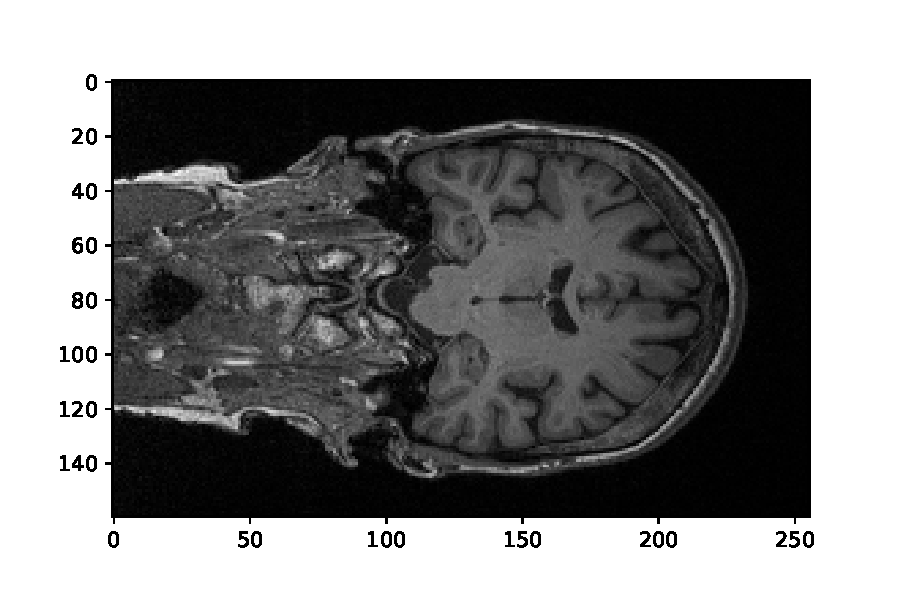
\includegraphics[height=.4\textwidth, trim={18 0 0 0}, clip]{images/preproc/raw.pdf}};
	\node[inner sep=0pt, anchor=north east] (fov) at (16.0, 0)
		{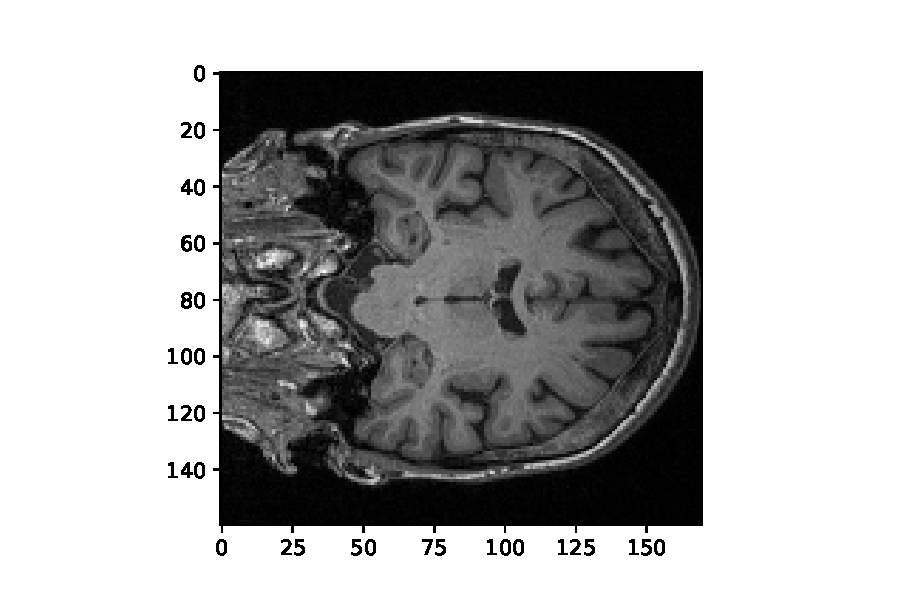
\includegraphics[height=.4\textwidth, trim={60 0 68 0}, clip]{images/preproc/fov.pdf}};
	
	\node[inner sep=0pt, anchor=north east] (fli) at (16.0, -5.75)
		{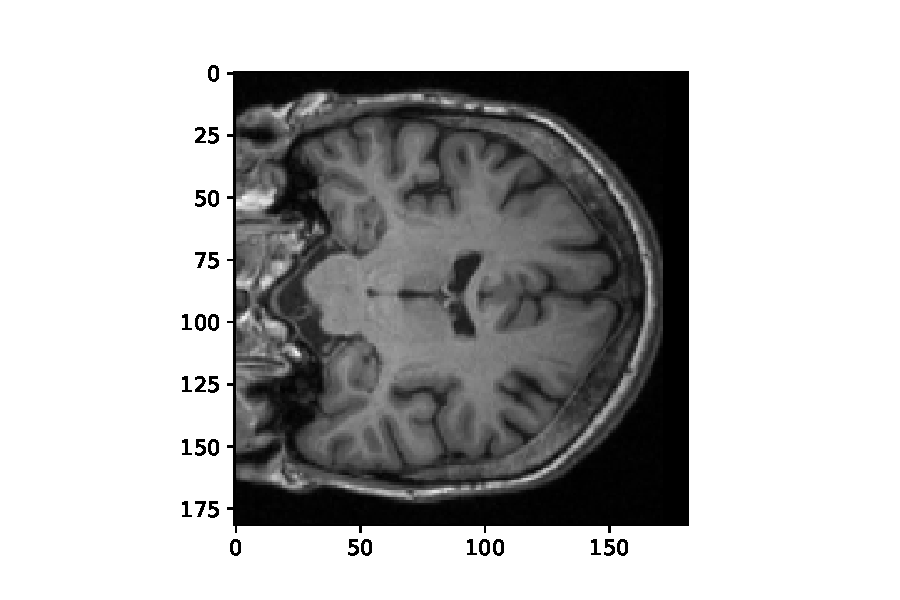
\includegraphics[height=.4\textwidth, trim={75 0 75 0}, clip]{images/preproc/fli.pdf}};
	\node[inner sep=0pt, anchor=north west] (msk) at ( 5.5, -5.75)
		{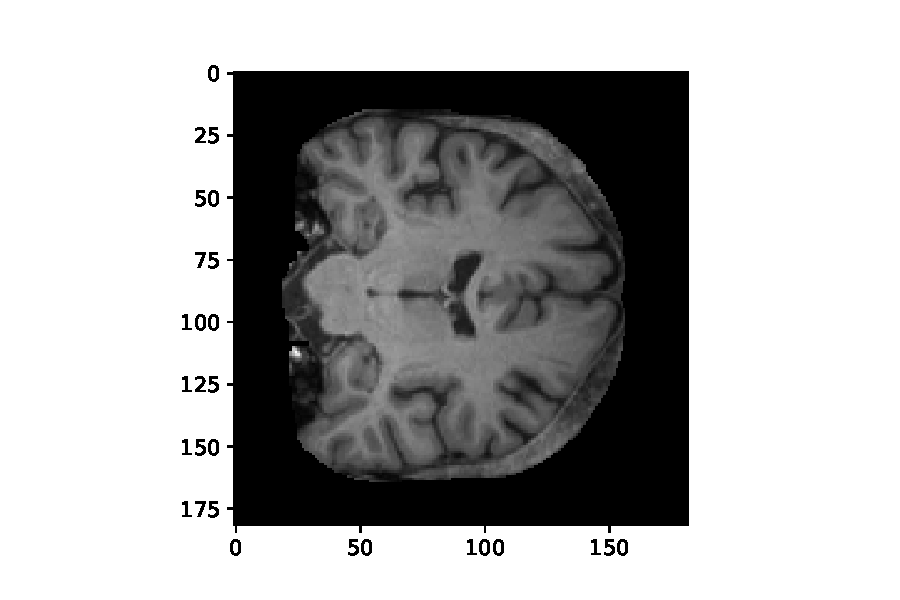
\includegraphics[height=.4\textwidth, trim={75 0 80 0}, clip]{images/preproc/msk.pdf}};
	\node[inner sep=0pt, anchor=north west] (bet) at ( 0.0, -5.75)
		{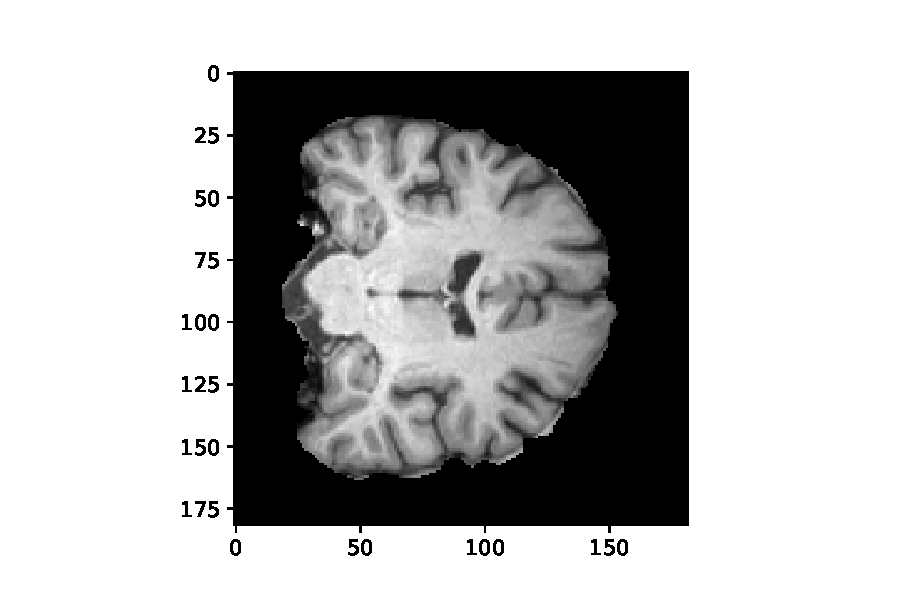
\includegraphics[height=.4\textwidth, trim={75 0 75 0}, clip]{images/preproc/bet.pdf}};

	\node[inner sep=0pt, anchor=north east] (pv1) at (16.0, -12)
		{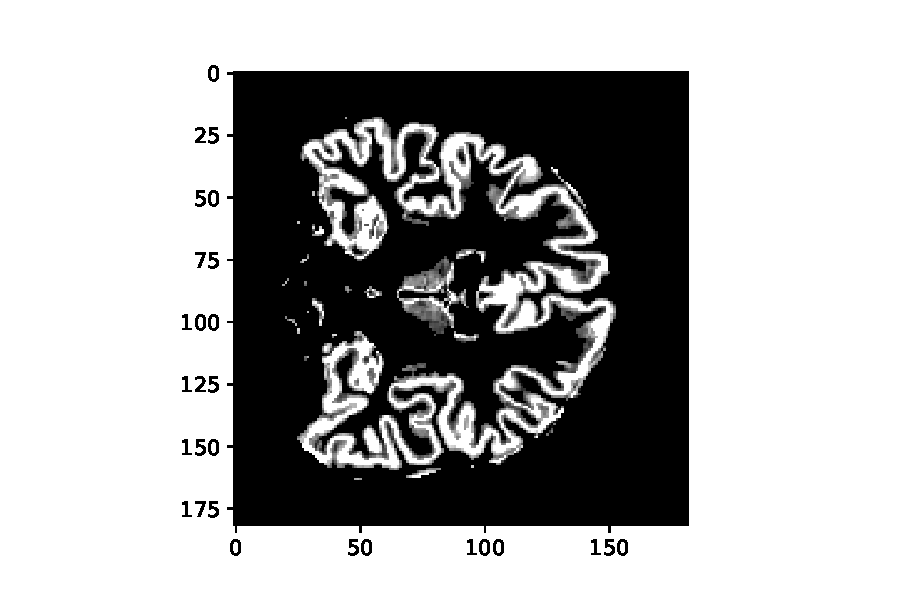
\includegraphics[height=.4\textwidth, trim={75 -10 75 10}, clip]{images/preproc/pve_1.pdf}};
	\node[inner sep=0pt, anchor=north west] (pv2) at ( 5.5, -12)
		{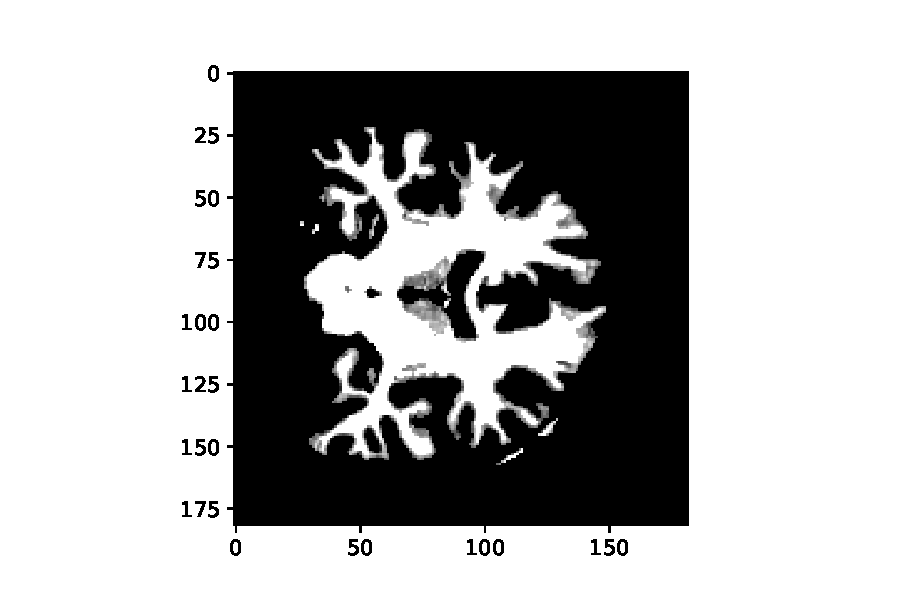
\includegraphics[height=.4\textwidth, trim={75 -10 75 10}, clip]{images/preproc/pve_2.pdf}};
	\node[inner sep=0pt, anchor=north west] (res) at ( 0.0, -12)
		{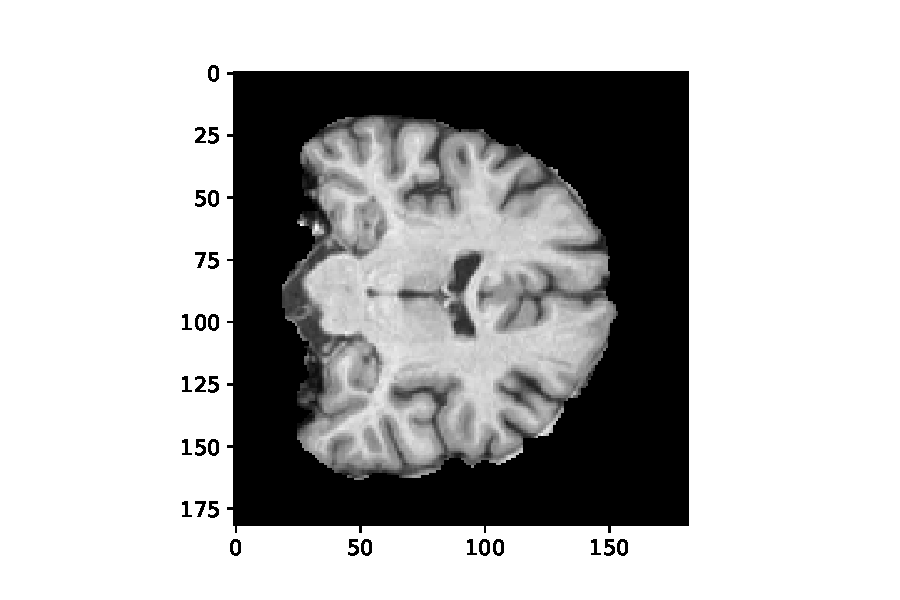
\includegraphics[height=.4\textwidth, trim={75 -10 75 10}, clip]{images/preproc/res.pdf}};
	
	\node[inner sep=0pt, anchor=north]      (sub) at (10.85, -17.75)
		{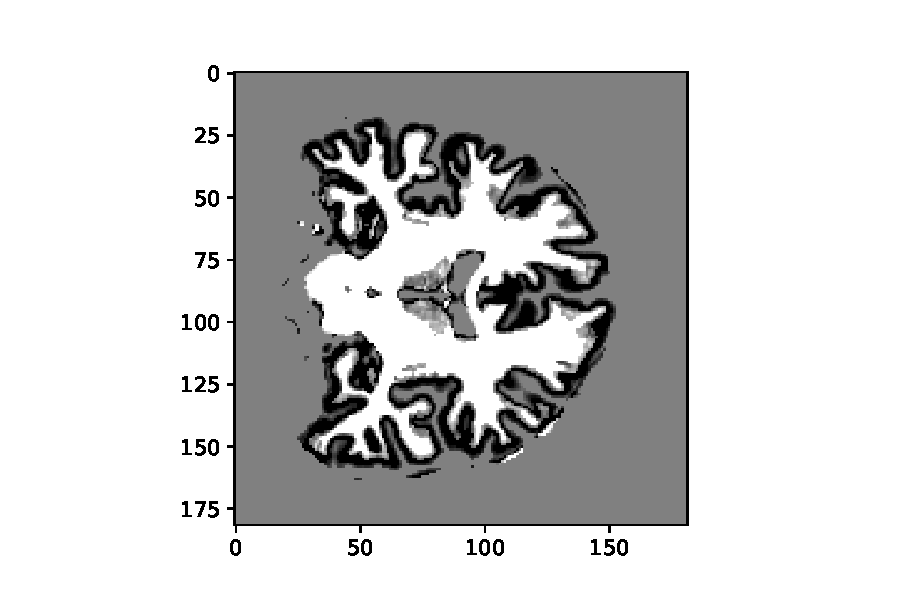
\includegraphics[height=.4\textwidth, trim={75 0 75 10}, clip]{images/preproc/sub.pdf}};

	\draw[->, very thick] (raw) -- node[below=5pt]{\texttt{robustfov}} (fov);
	\draw[->, very thick] (fov) -- node[right=10pt]{\texttt{flirt}} (fli);
	\draw[->, very thick] (fli) -- node[above=25pt, right=0pt, rotate=90]{\texttt{\ mask}} (msk);
	\draw[->, very thick] (msk) -- node[above=25pt, right=0pt, rotate=90]{\texttt{\ bet}}  (bet);
	\draw[->, very thick] (bet.south) -- (pv1.north);
	\draw[->, very thick] (bet.south) -- node[left=0pt, fill=white, inner sep=3pt]{\quad \texttt{fast}} (pv2.north);
	\draw[->, very thick] (bet.south) -- (res.north);
	\draw[->, very thick] (pv1) -- node[left=10pt]{\texttt{subtract}} (sub);
	\draw[->, very thick] (pv2) -- (sub);

	\node[below = -0.5 of res.south] (lres) {\small T1};
	\node[below = -0.5 of pv1.south] (lpv1) {\small WM};
	\node[below = -0.5 of pv2.south] (lpv2) {\small GM};


\end{tikzpicture}

	}
	\caption{Preprocessing pipeline visualized for one sample} \label{fig:preproc}
\end{figure}

Note that since the primary output of our preprocessing pipeline is based entirely on segmentation masks, one could combine the T1-weighted scans with data from different brain imaging modalities such as T2-weighted MRI data or proton density (PD) scans, therefore drastically increasing the number of possible data sources. However, we do not validate or pursue this idea in the context of this thesis.

For computational reasons, we also perform downsampling with a factor of 0.5 followed by cropping to keep only the center 32 coronal slices, resulting in a final shape of $ 80 \times 32 \times 80 $. However, note that our architecture uses 3D convolutions throughout and therefore can be trained on the unscaled data if desired, albeit at a significant computational penalty.

\subsection{Data Splitting} \label{sec:dat}
In order to run our experiments, we generate a number of data sets for the different settings. For the sake of notational brevity and consiceness, let $s$ denote one subject in our data set and let $v^s_i$ denote the $i$-th visit of subject s, with $V(s)$ denoting the temporally ordered set of visits $v^s_i \in V(s)$ of subject $s$, for $i \in 1 \ ..\ |V(s)|$. For redundancy, MRI scans are usually performed twice resulting in two separate but very similar images. Moreover, for some subjects images taken at different magnetic field strength levels are available. As a consequence, a visit $v^s_i$ typically consists of multiple images $x^s_{i, k} \in I(v^s_i)$ along with the corresponding image meta data. Finally, the examdate $t^s_i$ and the subject age $a^s_i$ at time $t^s_i$ as well as the diagnosis $d^s_i$ are available for most visits.

We split our data sets on a subject basis into training and validation sets containing roughly 80\% and 20\% of the data. This split is performed globally in the sense that given data sets $\mathcal{S}_a$ and $\mathcal{S}_b$, we have $\mathcal{S}_a^{train} \cap \mathcal{S}_b^{valid} = \varnothing$ and vice versa. In other words, a subject may only appear in either the training or validation split across all data sets.

\subsubsection*{Base Image Set} \label{sec:datsingles}
The \textit{Base Image Set} forms the foundation for all other data sets. It consists of all images $x^s_{i, j}$ and the meta data for the corresponding visits $v^s_i$ for which $t^s_i$ and $a^s_i$ are obtainable. We mainly use this set in the training of our age regressor models.

\subsubsection*{MCI/AD Set} \label{sec:datmciad}
The \textit{MCI/AD Set} consists of the images of all visits $v^s_i$ for which the diagnosis $d^s_i \in \{MCI, AD\}$ and we have high confidence in the label.

We consider a visit $v^s_i$ \textit{firmly MCI} if $d^s_i$ as well as both the diagnoses of the previous and following visit $d^s_{i-1}$ and $d^s_{i+1}$ are $MCI$. Implicitly, this also means that we only consider subjects with at least three visits. Conversely, for a visit $v^s_i$ to be considered \textit{firmly AD}, we require that both $d^s_i$ and $d^s_{i-1}$ are $AD$.

\subsubsection*{Image Pairs Set} \label{sec:datpairs}


\subsubsection*{MCI Conversion Set} \label{sec:datconv}
The \textit{MCI Conversion Set} consists of image pairs $(x^s_i, x^s_j)$ of progressive and stable MCI subjects according to the definitions in \autoref{sec:appconvpred}. Following the notation in \ref{sec:appconvpred}, we choose the time step between $x^s_i$ and $x^s_j$ to be $\Delta = 4$. In general, multiple viable image pair combinations exist for each subject and we prioritize matching $\Delta$ followed by centering the point in time where the diagnosis change occurs within $\Delta$.

\subsubsection*{Leave One Visit Out} \label{sec:datloo}
Finally, we prepare a data set of based on the image set using a different split for evaluation. 

\chapter{Experiments}

\section{Synthetic Data}
results without age reg

\section{Age Regressor} \label{sec:expagereg}
Validating the performance of a generative model is a hard problem in general. Beyond visual inspection of the outputs, we also pre-train an age regressor which given an image $x$ produces an estimated age label $\hat a_x$ and use it to estimate the age label of outputs generated by our model. Furthermore, the regressor is also included in the generator loss function as described in \autoref{sec:adaagereg}.

In this section, we present the results of our age regressor experiments. Given its importance in the validation of our generative model, we evaluate the its performance on a number of different tasks.

TODO(number of steps etc.)
TODO(multiple models? in appendix? multiple runs?)
TODO(weighted, non-weighted?)

\subsection*{Absolute Error}

\subsection*{Squared Error}

\subsection*{Delta Loss}


\section{Diagnosis Classifier}
We pre-train a diagnosis classifier to discriminate between images labeled as MCI and AD respectively. Given the gradual transition between the two diagnoses, we use the \textit{MCI/AD Set} described in \autoref{sec:datmciad}, which limits our training and validation sets to a subset of images with increased confidence in the diagnosis labels. Note that we use a binary classifier, that is we do not include or classifiy any subjects from the healthy control group HC, focussing instead on the more subtle distinctions between the MCI and AD diagnoses. We examine a number of different convolutional neural network architectures and report the results for three TODO(arbitrary, good idea?) of them. The models are trained on TODO(number of batches) X batches of size 64, corresponding to Y TODO(number of epochs) epochs on our training set. We train all models a total of three times to avoid local minima.

\section{Generator Models}

\subsection{Voxelmorph}

\subsection{Prediction}
TODO(predict brain at real delta)

\subsection{Fixed Time Step Prediction}
TODO(predict brain at fixed time step)
check resulting ages from age reg
plots plots plots
mention TI flow in passing, results were bad

\subsection{Long-Term Prediction}
AD/HC only, compare
also regular model? What to show? Age reg doesn't make much sense.

% subjects:
% AD:
% ADNI_1066	7	1.5	pMCI, 6 AD
% ADNI_922	7	1.5	pMCI, 6 AD
% ADNI_1427	7	1.5	pMCI, 7 AD

% HC:
% ADNI_382	8	1.5	
% ADNI_13	9	1.5
% ADNI_441	8	1.5
% ADNI_553	9	1.5
% ADNI_677	8	1.5
% ADNI_1098	9	1.5

% MCI:
% ADNI_925	11	1.5	pMCI, mostly MCI

with/without reg?

\section{Conversion Prediction}
F1 score, accuracy

We evalute our models ability to distinguish 

\chapter{Related Work}

\chapter{Discussion}
